
\section{Analisi dei Requisiti} \label{sec:analisi}
\subsection{Casi d'uso} %\label{sec:greetings}
In questa sezione verranno elencati i casi d'uso del sistema che è oggetto dello stage. Dato che il sistema è stato pensato per rispondere solo all'intervento di un utente che si occupa di amministrazione e installazione l'unico attore che prenderemo in considerazione è \textbf{utente}. Per ogni caso d'uso verranno riportate:
\begin{enumerate}
\item DESCRIZIONE: contenuto del caso d'uso
\item PRECONDIZIONI: asserzioni che sono valide prima dell'effettiva esecuzione del caso d'uso
\item POSTCONDIZIONI: asserzioni che sono valide dopo l'esecuzione del caso d'uso
\item SCENARI ALTERNATIVI: eventuali scenari alternativi che differiscono dal normale flusso del caso d'uso
\end{enumerate}
Ogni caso d'uso ha un identificativo stile UC\textit{n} dove n indica una posizione gerarchica.
Ogni caso d'uso è posizionato all'interno della gerarchia che parte dal caso d'uso più generale UC0 (radice dell'albero). Per ogni caso d'uso figlio valgono le precondizioni del padre.

\subsection{UC0: Scenario Principale}
\begin{description}
 \item[\em{descrizione}] L'utente può calibrare le telecamere, configurarle, oppure generare le statistiche a partire dai dati di tracking (figura ~\ref{fig:uc0})
 \item[\em{precondizione}] Il sistema è avviato e funzionante \end{description}
\begin{figure}[htpb]
\centering
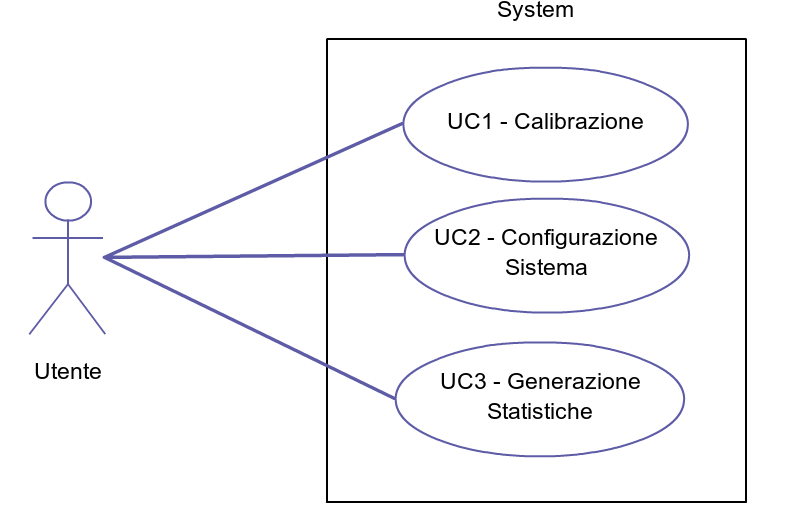
\includegraphics[scale=0.4]{./images/uc0.png}
\caption{UC0 - Scenario principale}
\label{fig:uc0}
\end{figure} 
 

\subsection{UC1: Calibrazione telecamere}
\begin{description}
 \item[\em{descrizione}] L'utente può calibrare le telecamere, o di visualizzare un video \textit{undistorted} che usa i parametri di calibrazione per correggere i frame. (figura ~\ref{fig:uc1})
 \item[\em{precondizione}] Il sistema è avviato e funzionante \end{description}
\begin{figure}[htpb]
\centering
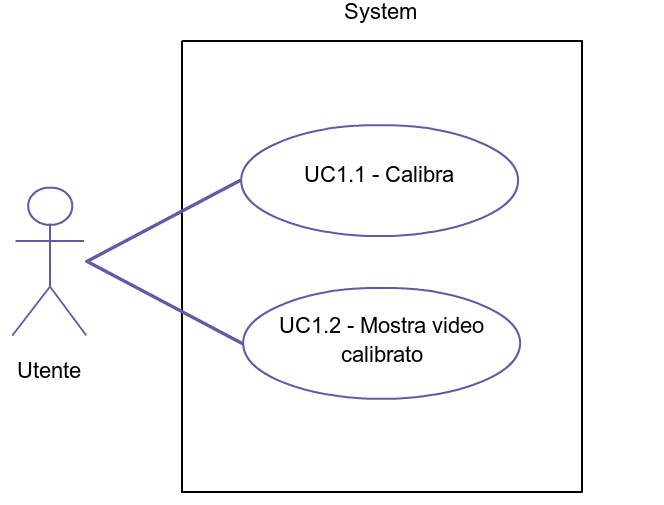
\includegraphics[scale=0.4]{./images/uc1.png}
\caption{UC1 - Calibrazione telecamere}
\label{fig:uc1}
\end{figure} 

\subsubsection{UC1.1: Calibra}
\begin{description}
 \item[\em{descrizione}] L'utente seleziona le opzioni per la calibrazione quali: numero di span spot, numero di frame da scartare, indirizzo della camera da calibrare, e poi inizia l'effettiva calibrazione.  (figura ~\ref{fig:uc1.1})
 \item[\em{postcondizione}] I file che contengono i file di
  calibrazione della telecamera (extrinsics e instrinsics) sono stati generati e salvati nel file system
  \item[\em{scenari alternativi}] L'utente interrompe la procedura, il sistema ritorna in attesa di eventi. \\
  La procedura fallisce, il sistema segnala l'errore e torna in attesa di eventi
 \end{description}
\begin{figure}[htpb]
\centering
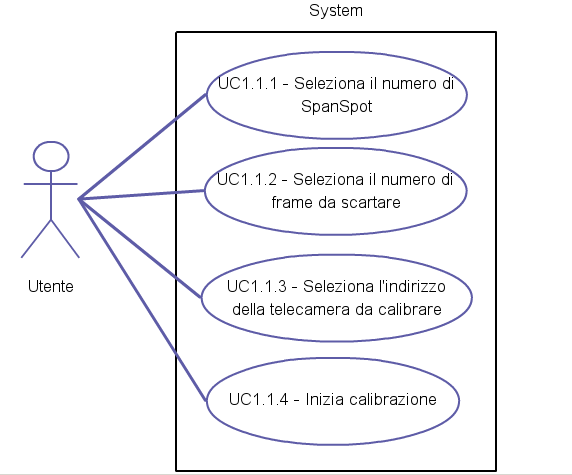
\includegraphics[scale=0.4]{./images/uc11.png}
\caption{UC1.1 - Calibra}
\label{fig:uc1.1}
\end{figure} 

\paragraph{UC1.1.1: Seleziona il numero di span spot}
\begin{description}
 \item[\em{descrizione}] L'utente seleziona il numero di span spot per la calibrazione
 \item[\em{postcondizione}] Il sistema conosce il numero di span spot da utilizzare nella calibrazione
  \item[\em{scenari alternativi}] L'utente interrompe la procedura, il sistema ritorna in attesa di eventi
 \end{description}

\paragraph{UC1.1.2: Seleziona il numero di frame da scartare}
\begin{description}
 \item[\em{descrizione}] L'utente seleziona il numero di frame da scartare per la calibrazione
 \item[\em{precondizione}] L'utente ha già selezionato il numero di span spot
 \item[\em{postcondizione}] Il sistema conosce il numero di frame da scartare nella calibrazione
  \item[\em{scenari alternativi}] L'utente interrompe la procedura, il sistema ritorna in attesa di eventi
 \end{description}

\paragraph{UC1.1.3: Inserisce l'indirizzo della telecamera da calibrare}
\begin{description}
 \item[\em{descrizione}] L'utente inserisce l'indirizzo della telecamera da calibrare
 \item[\em{precondizione}] L'utente ha già selezionato il numero di span spot e il numero di frame da scartare nella calibrazione
 \item[\em{postcondizione}] Il sistema conosce l'indirizzo della telecamera da calibrare
  \item[\em{scenari alternativi}] L'utente interrompe la procedura, il sistema ritorna in attesa di eventi
 \end{description}

\paragraph{UC1.1.4: Inizia calibrazione}
\begin{description}
 \item[\em{descrizione}] L'utente inizia la calibrazione effettiva
 \item[\em{precondizione}] L'utente ha già selezionato le opzioni di calibrazione (UC1.1.1 - UC1.1.2 - UC1.1.3), il sistema quindi conosce i parametri da utilizzare
 \item[\em{postcondizione}] Il sistema genera i file di calibrazione intrinsics ed extrinsics e li salva nel file system
  \item[\em{scenari alternativi}] La calibrazione non termina con successo quindi l'operazione viene interrotta e l'errore segnalato. Il sistema ritorna in attesa di eventi
 \end{description}


\subsection{UC2: Configurazione telecamere}
\begin{description}
 \item[\em{descrizione}] L'utente può impostare le opzioni di configurazione delle telecamere, aggiungendone di nuove, rimuovendole, modificandole, salvare un frame della telecamera per l'uso futuro, convertire un file .DXF in .PNG o calcolare la \textit{homography matrix} (figura ~\ref{fig:uc2})
 \item[\em{precondizione}] Il sistema è avviato e funzionante. \end{description}
\begin{figure}[htpb]
\centering
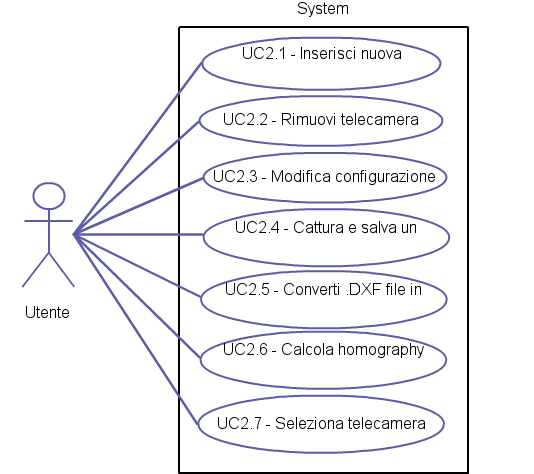
\includegraphics[scale=0.4]{./images/uc2.png}
\caption{UC2 - Configurazione telecamere}
\label{fig:uc2}
\end{figure} 

\subsubsection{UC2.1: Inserisci nuova}
\begin{description}
 \item[\em{descrizione}] L'utente inserisce il nome della nuova telecamera
 \item[\em{postcondizione}] Il sistema ha inserito la nuova telecamera nel database
 \item[\em{scenari alternativi}] Il nome inserito non è valido, il sistema interrompe l'operazione e torna in attesa di eventi.
 \end{description}

\subsubsection{UC2.2: Rimuovi telecamera}
\begin{description}
 \item[\em{descrizione}] L'utente rimuove la telecamera selezionata
  \item[\em{precondizione}] L'utente ha selezionato una telecamera tra quelle esistenti
 \item[\em{postcondizione}] Il sistema ha rimosso la telecamera dal database
 \end{description}
 
\subsubsection{UC2.3: Modifica configurazione}
\begin{description}
 \item[\em{descrizione}] L'utente modifica le opzioni di configurazione della telecamera selezionata, quali: file extrinsics, intrinsics, valore dell'altezza del frame, valore della larghezza del frame, percorso del file contentente la \textit{homography matrix} (figura ~\ref{fig:uc23}).
  \item[\em{precondizione}] L'utente ha selezionato una telecamera tra quelle esistenti
  \item[\em{scenari alternativi}] L'utente interrompe la modifica, il sistema ritorna in attesa di eventi
 \end{description}
 \begin{figure}[htpb]
\centering
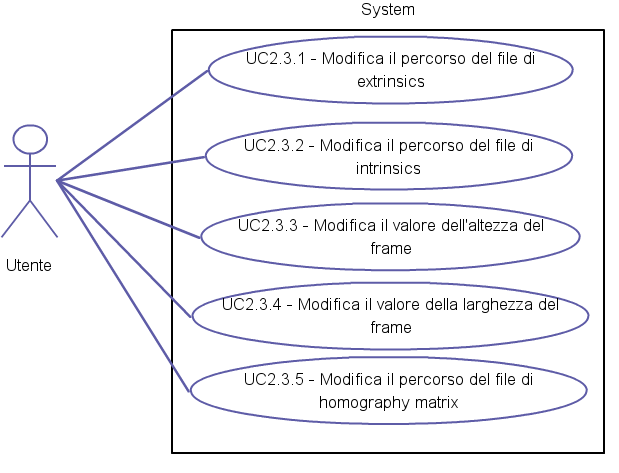
\includegraphics[scale=0.4]{./images/uc23.png}
\caption{UC2.3 - Modifica telecamere}
\label{fig:uc23}
\end{figure} 

\paragraph{UC2.3.1: Modifica il percorso del file di extrinsics}
\begin{description}
 \item[\em{descrizione}] L'utente seleziona un file nel file system che contiene i valori \textit{extrinsics} di calibrazione.
   \item[\em{postcondizione}] Il sistema ha modificato il corrispondente valore della telecamera nel database
  \item[\em{scenari alternativi}] L'utente interrompe la selezione, il sistema ritorna in attesa di eventi
 \end{description}

\paragraph{UC2.3.2: Modifica il percorso del file di intrinsics}
\begin{description}
 \item[\em{descrizione}] L'utente seleziona un file nel file system che contiene i valori \textit{intrinsics} di calibrazione.
   \item[\em{postcondizione}] Il sistema ha modificato il corrispondente valore della telecamera nel database
  \item[\em{scenari alternativi}] L'utente interrompe la selezione, il sistema ritorna in attesa di eventi
 \end{description}

\paragraph{UC2.3.3: Modifica il valore dell'altezza del frame}
\begin{description}
 \item[\em{descrizione}] L'utente seleziona un valore per l'altezza del frame della telecamera.
   \item[\em{postcondizione}] Il sistema ha modificato il corrispondente valore della telecamera nel database
 \end{description}
 
\paragraph{UC2.3.4: Modifica il valore della larghezza del frame}
\begin{description}
 \item[\em{descrizione}] L'utente seleziona un valore per la larghezza del frame della telecamera.
   \item[\em{postcondizione}] Il sistema ha modificato il corrispondente valore della telecamera nel database
 \end{description}
 
 \paragraph{UC2.3.5: Modifica il percorso del file di homography matrix}
\begin{description}
 \item[\em{descrizione}] L'utente seleziona un file nel file system che contiene i valori che descrivono la  \textit{homography matrix} utilizzata per la traduzione delle coordinate.
   \item[\em{postcondizione}] Il sistema ha modificato il corrispondente valore della telecamera nel database
  \item[\em{scenari alternativi}] L'utente interrompe la selezione, il sistema ritorna in attesa di eventi
 \end{description}
 
\subsection{UC3: Generazione statistiche}
\begin{description}
 \item[\em{descrizione}] L'utente può visualizzare le statistiche relative ai dati presenti nel sistema. Può effettuare la conversione dei dati \textit{raw}, visualizzare l'\textit{heatmap}, o le statistiche (figura ~\ref{fig:uc3})
 \item[\em{precondizione}] Il sistema è avviato e funzionante.
  \end{description}
\begin{figure}[htpb]
\centering
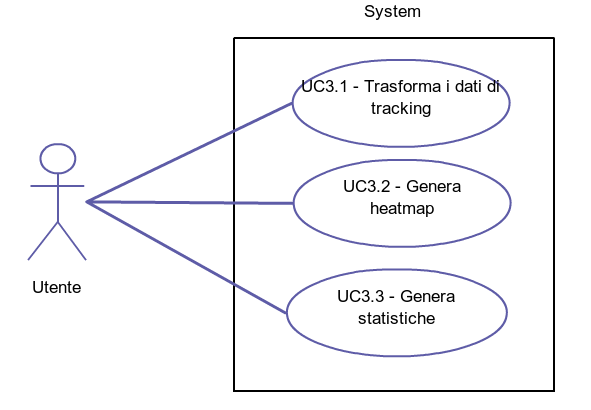
\includegraphics[scale=0.4]{./images/uc3.png}
\caption{UC2 - Generazione statistiche}
\label{fig:uc3}
\end{figure}  
 
\subsubsection{UC3.1: Trasforma i dati di tracking}
\begin{description}
 \item[\em{descrizione}] L'utente indica al sistema di eseguire la trasformazione dei dati \textit{raw} di tracking
  \item[\em{postcondizione}] Il sistema ha trasformato i dati presenti nel database ed ha salvato i dati trasformati.
  \end{description}
  
\subsubsection{UC3.2: Genera heatmap}
\begin{description}
 \item[\em{descrizione}] L'utente indica al sistema di generare l'heatmap con la rappresentazione grafica dei dati di tracking
  \item[\em{postcondizione}] Il sistema elabora i dati presenti nel database generando l'heatmap e salvandola nel file system.
  \item[\em{scenari alternativi}] La generazione fallisce, il sistema segnala l'errore e torna nello stato di attesa.
  \end{description}
  
\subsection{Requisiti}